\documentclass[12pt]{article}
\usepackage[margin=1in]{geometry} 
\usepackage{amsmath}
\usepackage{amssymb}
\usepackage{siunitx}
\usepackage{float}
\usepackage{tikz}
\def\checkmark{\tikz\fill[scale=0.4](0,.35) -- (.25,0) -- (1,.7) -- (.25,.15) -- cycle;} 
\usepackage{url}
\usepackage[siunitx,american,RPvoltages]{circuitikz}
\ctikzset{capacitors/scale=0.7}
\ctikzset{diodes/scale=0.7}
\usepackage{tabularx}
\newcolumntype{C}{>{\centering\arraybackslash}X}
\renewcommand\tabularxcolumn[1]{m{#1}}% for vertical centering text in X column
\usepackage{tabu}
\usepackage[spanish,es-tabla,activeacute]{babel}
\usepackage{babelbib}
\usepackage{booktabs}
\usepackage{pgfplots}
\usepackage{hyperref}
\hypersetup{colorlinks = true,
            linkcolor = black,
            urlcolor  = blue,
            citecolor = blue,
            anchorcolor = blue}
\usepgfplotslibrary{units, fillbetween} 
\pgfplotsset{compat=1.16}
\usepackage{bm}
\usetikzlibrary{arrows, arrows.meta, shapes, 3d, perspective, positioning,mindmap,trees,backgrounds}
\renewcommand{\sin}{\sen} %change from sin to sen
\usepackage{bohr}
\setbohr{distribution-method = quantum,insert-missing = true}
\usepackage{elements}
\usepackage{verbatim}
\usepackage[edges]{forest}
\usepackage{etoolbox}
\usepackage{schemata}
\usepackage{appendix}
\usepackage{listings}

\definecolor{color_mate}{RGB}{255,255,128}
\definecolor{color_plas}{RGB}{255,128,255}
\definecolor{color_text}{RGB}{128,255,255}
\definecolor{color_petr}{RGB}{255,192,192}
\definecolor{color_made}{RGB}{192,255,192}
\definecolor{color_meta}{RGB}{192,192,255}
\newcommand\diagram[2]{\schema{\schemabox{#1}}{\schemabox{#2}}}

\definecolor{codegreen}{rgb}{0,0.6,0}
\definecolor{codegray}{rgb}{0.5,0.5,0.5}
\definecolor{codepurple}{rgb}{0.58,0,0.82}
\definecolor{backcolour}{rgb}{0.95,0.95,0.92}

\lstdefinestyle{mystyle}{
    backgroundcolor=\color{backcolour},   
    commentstyle=\color{codegreen},
    keywordstyle=\color{magenta},
    numberstyle=\tiny\color{codegray},
    stringstyle=\color{codepurple},
    basicstyle=\ttfamily\footnotesize,
    breakatwhitespace=false,         
    breaklines=true,                 
    captionpos=b,                    
    keepspaces=true,                 
    numbers=left,                    
    numbersep=5pt,                  
    showspaces=false,                
    showstringspaces=false,
    showtabs=false,                  
    tabsize=2
}

\lstset{style=mystyle}
\usepackage{lastpage}
\usepackage{fancyhdr}
\pagestyle{fancy}
\setlength{\headheight}{42pt}
\setlength{\parindent}{0cm}
 
\begin{document}
\sisetup{unit-math-rm=\mathrm,math-rm=\mathrm} % change sinitx font
\sisetup{output-decimal-marker = {,}}
\lhead{Ingeniería en Mantenimiento Industrial \\ Escuela de Ingeniería Electromecánica \\ Tecnológico de Costa Rica} 
\rhead{Electricidad I \\ Tarea \#3  \\ Entrega: Semana 13} 
\cfoot{\thepage\ de \pageref{LastPage}}

Definiciones:
\begin{itemize}
    \item Celda fotovoltaica o celda solar: es un dispositivo capaz de convertir la energía solar en energía eléctrica por medio del efecto fotoeléctrico. 
    \item Panel fotovoltaico o panel solar: es la interconexión de dos o mas celdas solares montadas en una estructura que les da soporte mecánico. 
    \item Irradiancia solar (\si{\watt\meter^{-2}}): es la potencia por unidad de superficie que se recibe del sol en forma de radiación electromagnética.
    \item Constante solar (\si{\watt\meter^{-2}}): es la irradiancia medida en la parte externa de la atmósfera terrestre y en una superficie perpendicular a los rayos del sol.
    \item Ángulo de incidencia (\si{\degree}): es el ángulo entre los rayos del sol y la normal de una superficie en el punto de incidencia. 
\end{itemize}

Existe gran diversidad de modelos para paneles solares, uno de los modelos mas comunes es el de \emph{un diodo}, también conocido como el de \emph{5 parámetros}. En la Figura \ref{fig:OneDiode} se muestra este modelo. 

\begin{figure}[H]
    \centering
    \begin{circuitikz}
        \draw 
        (0,0)
            to[cI, l=$I_L$]
        (0,3)
            to[short]
        (3,3)
            to[R,l=$R_s$, i=$I$, -o]
        (6,3)
            to[open, v=$v$, voltage shift = -0.1cm]
        (6,0)
            to[short, o-]
        (0,0)
        (1.5,3)
            to[D,i=$I_{D}$]
        (1.5,0)
        (3,3)
            to[R,l=$R_{sh}$, i=$I_{sh}$]
        (3,0)
        ;
    \end{circuitikz}
    \caption{Modelo de un diodo para celda fotovoltaica}
    \label{fig:OneDiode}
\end{figure}

\tikzstyle{line} = [draw, very thick, {Circle[length=4pt]}-latex',shorten <=-2pt]
\begin{figure}[H]
    \centering
    \begin{tikzpicture}
        \begin{axis}[
            %yshift=-1cm,
            width=8cm, % Scale the plot to \linewidth
            height=6cm,
            %grid=major, % Display a grid
            %grid style={dashed,gray!30}, % Set the style
            every axis plot/.append style={thick},
            ymin=0, ymax=2,
            xmin=0, xmax=6,
            axis x line=bottom,
            axis y line=left,
            axis line style={-},
            xtick align=inside,
            ytick align=inside,
            xlabel=Voltaje, % Set the labels
            ylabel=Potencia,
            x unit=V, 
            y unit=A,
            legend pos=north east,
            legend cell align={left},
            %legend style={cells={anchor=west}}
            legend style={at={(1.4,0.5)},anchor=east}, % Put the legend below the plot
            smooth,
            ]
            \addplot [mark=none,color=red!0!blue]       
            table[x=V,y=I,col sep=comma] {../data/real_solar_panel.csv};
            %\addlegendentry{Begining of life};
        \end{axis}
        \begin{axis}[
            xshift=8cm,
            width=8cm, % Scale the plot to \linewidth
            height=6cm,
            %grid=major, % Display a grid
            %grid style={dashed,gray!30}, % Set the style
            every axis plot/.append style={thick},
            ymin=0, ymax=8,
            xmin=0, xmax=6,
            axis x line=bottom,
            axis y line=left,
            axis line style={-},
            xtick align=inside,
            ytick align=inside,
            xlabel=Voltaje, % Set the labels
            ylabel=Potencia,
            x unit=V, 
            y unit=W,
            legend pos=north east,
            %legend style={cells={anchor=west}}
            legend cell align={left},
            legend style={at={(1.4,0.5)},anchor=east}, % Put the legend below the plot
            %x tick label style={rotate=90,anchor=east}, % Display labels sideways
            ]
            \addplot [mark size=2pt, color=red!0!blue]       
            table[x=V,y=P,col sep=comma] {../data/real_solar_panel.csv};
            %\addlegendentry{Begining of life};
        \end{axis}
    \end{tikzpicture}
    \caption{Curvas I-V y P-V de la celda 3G30A usando el método de Villalva}
    \label{fig:real_plots}
\end{figure}

Existen gran cantidad de métodos para determinar los cinco parámetros y con ellos darle valores a los elementos del circuito mostrado en la Figura \ref{fig:OneDiode}; sin embargo, todos ellos están fuera del alcance de este curso. El método desarrollado por Villava \cite{villalva2009modeling} permite construir el modelo usando la información que se puede encontrar en la hoja de datos de la celda. Si usamos este método con un arreglo de 2 celdas en serie y 3 en paralelo (2s3p), usando la celda modelo 3G30A de Azurspace (ver Figura \ref{fig:3G30A}), obtendríamos una curva similar a la de la Figura \ref{fig:real_plots}. Esto es a una temperatura de $\SI{28}{\celsius}$, una irradiación igual a la constante solar, osea $\SI{1367}{\watt\meter^{-2}}$ y al inicio de su vida útil (BOL, beginning of life). Los datos importantes para poder construir el modelo de un arreglo 2s3p están en la Tabla \ref{t:cell}

\begin{figure}[H]
    \centering
    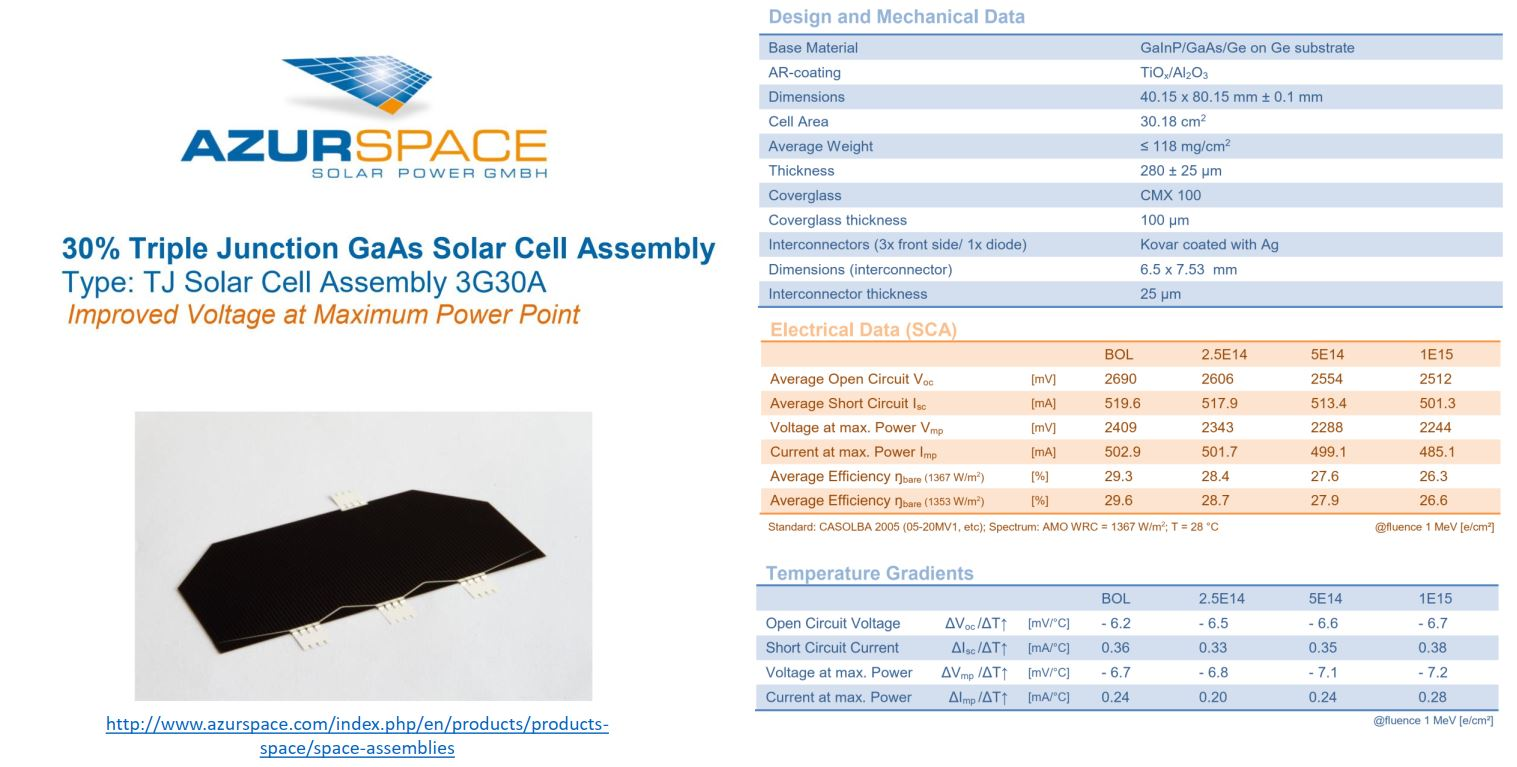
\includegraphics[width=0.95\linewidth]{fig/3G30A.JPG}
    \caption{Extracto de la hoja de datos del fabricante para celda 3G30A de Azurspace, tomado de \url{http://www.azurspace.com/images/products/0003401-01-01_DB_3G30A.pdf}}
    \label{fig:3G30A}
\end{figure}

\begin{table}[H]
	\footnotesize
	\centering
	\caption{Arreglo 2s3p con Azurspace 3G30A}
	\vspace{0.2cm}
	\begin{tabular}{ccc} 
		\toprule
		\textbf{Configuración ->} & \textbf{1 celda} & \textbf{2s3p (6 celdas)} \\
		\midrule
		$V_{oc}$ (V) & 2.69 & 5.38 \\
		$I_{sc}$ (A) & 0.52 & 1.56 \\
		$V_{mp}$ (V) & 2.41 & 4.82 \\
		$I_{mp}$ (A) & 0.50 & 1.51 \\ 
		\bottomrule
    \end{tabular}
    \label{t:cell}
\end{table}

Un forma muy simplificada de modelar esta misma celda se puede realizar usando dos rectas, tal como se muestra en la Figura \ref{fig:flat_plots} en la que se incluyen las curvas de la Figura \ref{fig:real_plots} en gris discontinuo. En este caso la curva I-V se puede construir usando lineas rectas entre las siguientes tres coordenadas: $(0,I_{sc}) - (V_{mp}, I_{mp}) - (V_{oc},0)$ y el modelo sería solamente una fuente de corriente dependiente del voltaje entre sus propias terminales. 

\begin{figure}[H]
    \centering
    \begin{circuitikz}
        \draw 
        (0,0)
            to[cI, l=$I(v)$]
        (0,3)
            to[short,-o]
        (3,3)
            to[open, v=$v$, voltage shift = -0.1cm]
        (3,0)
            to[short, o-]
        (0,0)
        ;
    \end{circuitikz}
    \caption{Modelo simplificado de dos rectas para celda fotovoltaica}
    \label{fig:simple}
\end{figure}

\begin{figure}[H]
    \centering
    \begin{tikzpicture}
        \begin{axis}[
            %yshift=-1cm,
            width=8cm, % Scale the plot to \linewidth
            height=6cm,
            %grid=major, % Display a grid
            %grid style={dashed,gray!30}, % Set the style
            every axis plot/.append style={thick},
            ymin=0, ymax=2,
            xmin=0, xmax=6,
            axis x line=bottom,
            axis y line=left,
            axis line style={-},
            xtick align=inside,
            ytick align=inside,
            xlabel=Voltaje, % Set the labels
            ylabel=Corriente,
            x unit=V, 
            y unit=A,
            legend pos=north east,
            legend cell align={left},
            %legend style={cells={anchor=west}}
            legend style={at={(1.4,0.5)},anchor=east}, % Put the legend below the plot
            smooth,
            ]
            \addplot [mark=none,color=gray, dashed]       
            table[x=V,y=I,col sep=comma] {../data/real_solar_panel.csv};
            %\addlegendentry{Begining of life};
            \addplot [mark=none, color=red!100!blue, sharp plot]       
            table[x=V,y=I,col sep=comma] {../data/flat_solar_panel.csv};
            %\addlegendentry{Begining of life};
        \end{axis}
        \begin{axis}[
            xshift=8cm,
            width=8cm, % Scale the plot to \linewidth
            height=6cm,
            %grid=major, % Display a grid
            %grid style={dashed,gray!30}, % Set the style
            every axis plot/.append style={thick},
            ymin=0, ymax=8,
            xmin=0, xmax=6,
            axis x line=bottom,
            axis y line=left,
            axis line style={-},
            xtick align=inside,
            ytick align=inside,
            xlabel=Voltaje, % Set the labels
            ylabel=Potencia,
            x unit=V, 
            y unit=W,
            legend pos=north east,
            %legend style={cells={anchor=west}}
            legend cell align={left},
            legend style={at={(1.4,0.5)},anchor=east}, % Put the legend below the plot
            %x tick label style={rotate=90,anchor=east}, % Display labels sideways
            ]
            \addplot [mark size=2pt, color=gray,dashed]       
            table[x=V,y=P,col sep=comma] {../data/real_solar_panel.csv};
            %\addlegendentry{Begining of life};
            \addplot [mark size=2pt, color=red!100!blue, sharp plot]       
            table[x=V,y=P,col sep=comma] {../data/flat_solar_panel.csv};
            %\addlegendentry{Begining of life};
        \end{axis}
    \end{tikzpicture}
    \caption{Curvas I-V y P-V de la celda 3G30A usando líneas rectas}
    \label{fig:flat_plots}
\end{figure}

Tomando en cuenta todo lo anterior, en esta tarea se procederá a realizar un proceso de carga de una celda NCR18650B (ya modelada en la Tarea \#2) usando el circuito de la Figura \ref{fig:carga}. 

\begin{figure}[H]
    \centering
    \begin{circuitikz}
        \draw 
        (0,0)
            to[cV, l=OCV$(z)$]
        (0,3)
            to[R, l=$R_0$,i=$i(t)$,-o]
        (3,3)
            to[open,v^=$v(t)$]
        (3,0)
            to[short,o-]
        (0,0)
        (3,3) 
            to[short]
        (6,3)
            to[cI, l=$I(v)$, invert]
        (6,0)
            to[short]
        (3,0)
        ;
    \end{circuitikz}
    \caption{Circuito para carga una celda electroquímica usando un panel solar}
    \label{fig:carga}
\end{figure}

\textbf{Instrucciones}
\begin{enumerate}
    \item Utilice las funciones y resultados obtenidos en la Tarea \#2 donde sean necesarios. 
    \item Asuma un panel con las siguientes características $I_{sc} = \SI{1.05}{\ampere}$, $V_{mp}=\SI{3.8}{\volt}$, $I_{mp}=\SI{1}{\ampere}$,  $V_{oc}= \SI{4}{\volt}$. 
    \item Defina la función en partes $I(v)$ usando los valores anteriores. Pista \#1: $y=mx+b$. Pista \#2: es posible mover el eje de las ordenadas y redefinir la variable independiente para facilitar la determinación de la ecuación de una recta. Incluya las ecuaciones que definen la función en partes en el informe. 
    \item Asuma que $Q = \SI{3250}{\milli\ampere\hour}$, $z(t_0) = 0.20$, $R_0 = \SI{100}{\milli\ohm}$ y $\eta = 0.98$. Considere un proceso en el que la celda se carga hasta que la corriente es sea igual a \SI{100}{\milli\ampere}, puede asumir que la corriente en el primer instante es $I_{sc}$, luego de resolver el problema por primera vez, puede sustituir este valor por la corriente en el segundo instante y volver a correr la solución.
    \item Usando Python cree un \emph{script} llamado ``calculos'' que le permita realizar lo siguiente:
    \begin{itemize}
        \item crear una función que permita ingresar cualquier valor de $v$ y recibir el valor correspondiente de $I(v)$ con base en las ecuaciones determinadas en el punto 2.
        \item programar el proceso de carga descrito en el punto 2 usando los conceptos y leyes básicas vistos en el curso, aproximando la integral que describe $z(t)$ por medio de una discretización con un intervalo de \SI{0.1}{\second}, esto es: 
        \begin{equation*}
            z[k+1] = z[k] - \dfrac{\eta \Delta t}{Q}i[k]
        \end{equation*}
        donde $\Delta t$ es el intervalo de integración discreta, en este caso \SI{0.1/3600}{\hour}; $z[k]$ e $i[k]$ son los valores actuales del SOC y la corriente respectivamente; y $z[k+1]$ es el valor siguiente del SOC
        \item generar una gráfica que en las abscisas tenga los valores del tiempo $t$ y en las ordenadas tenga el valor del voltaje $v(t)$
        \item generar una gráfica que en las abscisas tenga los valores del tiempo $t$ y en las ordenadas tenga el valor de la corriente $i(t)$. 
        \item generar una gráfica que en las abscisas tenga los valores del tiempo $t$ y en las ordenadas tenga el valor del SOC $z(t)$.
        \item imprimir en la terminal el valor del SOC inicial, SOC al final de la carga, la capacidad cargada y el tiempo transcurrido. Incluya estos resultados en el informe.
    \end{itemize}
    \item Responda la siguiente pregunta en el informe: Cuál es el voltaje máximo al que se puede cargar la celda electroquímica usando este panel solar de 2s3p? Justifique su respuesta.
    \item Realice un informe de su tarea llamado ``Informe\_t3.pdf'' usando \LaTeX. Incluya todos los cálculos y las gráficas solicitadas y algún texto complementario que permita entender la solución realizada. Un machote se puede encontrar \href{https://www.overleaf.com/read/phnwtckqwqwc}{acá}
    \item Comprima todo en un solo archivo .zip y suba al TecDigital. Cualquier entrega tardía se califica con base en 70. 
\end{enumerate}

\bibliographystyle{IEEEtran}
\bibliography{ref_tareas}

\end{document}